% ------------------------------------------
%  MASTER THESIS DISSERTATION
% ------------------------------------------
% Author:
%
% Advisors:
%
% ------------------------------------------
\documentclass[10pt,twoside,openright,a4paper]{report}
\usepackage[utf8]{inputenc}

% Set document margins to 1in in all sides
\usepackage[margin=2.5cm]{geometry}
% Line spacing package
\usepackage{graphicx, helvet, hyperref, setspace}
\usepackage[portuguese,english]{babel}
\usepackage[nomain, acronym, toc]{glossaries}
% Extra stuff file
% This file is included before begin{document} environment
% Use this to include extra packages and define your own commands
% This way, you can easily grab a most recent version
% of dissertation.tex file from the original repo

\usepackage{caption}
% Built the glossary when the main file is built.
\makeglossaries
% Set main font to Arial
\renewcommand{\familydefault}{\sfdefault}
% Define keywords macro
\providecommand{\keywords}[1]{\textbf{Keywords:} #1}
% Define "palavras-chave" macro
\providecommand{\palavrasChave}[1]{\textbf{Palavras-Chave:} #1}
% Define the NewPage macro
\newcommand*\NewPage{\newpage\null\thispagestyle{empty}\cleardoublepage}
% Abstract-en page numbering
\newcommand {\abstractEnglishPageNumber} {\thispagestyle{plain}\setcounter{page}{\abstractEnglishPage}}
% Abstract-pt page numbering
\newcommand {\abstractPortuguesePageNumber} {\thispagestyle{plain}\setcounter{page}{\abstractPortuguesePage}}
% Section numbering depth
\setcounter{secnumdepth}{3}
% Table of contents depth
\setcounter{tocdepth}{3}
% Set line spacing to 1.5cm
\onehalfspacing
% Page numbering
\pagestyle{plain}

% Glossary-File
% Glossary Definition

\newglossaryentry{MSc}{name={MSc}, description={Masters degree in the area of Science.}}

% Acronym-File
% Acronym Definition

\newacronym{IST}{IST}{Instituto Superior T\'ecnico}
\newacronym{CAD}{CAD}{Computer Aided Design}
\newacronym{GD}{GD}{Generative Design}
\newacronym{CPU}{CPU}{Central Processing Unit}
\newacronym{GPU}{GPU}{Graphics Processing Unit}
\newacronym{PL}{PL}{Programming Language}
\newacronym{VL}{VL}{Visualization Library}
\newacronym{API}{API}{Application Programming Interface}

\newacronym{HD}{HD}{High-Definition}
\newacronym{VR}{VR}{Virtual Reality}

\newacronym{LOD}{LOD}{Level of Detail}
\newacronym{OC}{OC}{Occlusion Culling}


% ------------------------------------------
% MASTER THESIS DISSERTATION
% ------------------------------------------

\begin{document}
\pagenumbering{gobble}% Remove page numbers (and reset to 1)
\clearpage
\thispagestyle{empty}
%!TEX root = ./dissertation.tex

% Dissertation basic information
\newcommand {\Title} {Fast Visualization of Large Architectural Models}
\newcommand {\Subtitle} {My Subtitle}
\newcommand {\StudentName} {Artur José Brás Mayer Alkaim}
\newcommand {\DegreeName} {Information Systems and Computer Engineering}
\newcommand {\Supervisors} { António Paulo Teles de Menezes Correia Leitão}

% Include or not include acknowledgments
\def \includeAcknowledgments{1}

% Include or not include glossary
\def \includeGlossary{0}

% Examination Committee
\newcommand {\Advisor} {{\large Prof./Dr. António Paulo Teles de Menezes Correia Leitão}}
\newcommand {\CoAdvisor} {{\large Prof./Dr. Co Advisor}}

% After the thesis defense
\newcommand {\CommitteeMembers} {
{\large Prof./Dr. João António Madeiras Pereira}\\
{\large Prof./Dr. Lorem Ipsum}
}
\newcommand {\Chairperson} {{\large Prof./Dr. Lorem Ipsum}}

% Is final version (will include Committee Members information)
\def \IsFinalVersion{1}

% Date
\newcommand {\Month} {October}
\newcommand {\Year} {2015}

% Acknowledgments page number
\def \acknowledgmentsPage{1}

% Abstract-en page numbering
\def \abstractEnglishPage{3}

% Abstract-pt page number
\def \abstractPortuguesePage{5}

% You had a co-advisor:
\def \HasCoAdvisor{0}

% Logo Spacing Variables
\def \finalLogoSpacing{2.0cm}
\def \draftLogoSpacing{2.0cm}

% Advisors Spacing Variables
\def \finalAdvisorsSpacing{1.0cm}
\def \draftAdvisorsSpacing{10.0cm}

% Date Spacing Variable
\def \dateSpacing{5.0cm}

% You can define your own variables here


%!TEX root = ./dissertation.tex

% ---------------------------------------------------------
%   MASTER THESIS DISSERTATION COVER
% ---------------------------------------------------------
\begin{titlepage}
% ---------------------------------------------------------
%  INSTITUTION LOGO
% ---------------------------------------------------------

\includegraphics[width=5cm]{images/ist_logo}~\\
%
\if\IsFinalVersion 1
  \vspace*{\finalLogoSpacing}
\else
  \vspace*{\draftLogoSpacing}
\fi

\begin{center}
% ---------------------------------------------------------
%  MASTER THESIS DISSERTATION TITLE
% ---------------------------------------------------------
{\LARGE \textbf{\Title}}\\[1.0cm]
% ---------------------------------------------------------
%  MASTER THESIS DISSERTATION SUBTITLE
% ---------------------------------------------------------
%{\Large \Subtitle}\\[1.0cm]
% ---------------------------------------------------------
%  AUTHOR NAME (FULL)
% ---------------------------------------------------------
{\Large \textbf{\StudentName}}\\[1.0cm]
% ---------------------------------------------------------
%  DISSERTATION DEGREE
% -----------------------------------------------------------------
{\large Thesis to obtain the Master of Science Degree in}\\[1.0cm]
% -----------------------------------------------------------------
%  COURSE NAME
% -----------------------------------------------------------------
{\LARGE \textbf{\DegreeName}}\\[1.0cm]

% -----------------------------------------------------------------
%  ADVISORS NAME
% ---------------------------------------------------------
%\begin{minipage}[t]{.5\textwidth}
%  \begin{flushright}
%    {\large Supervisor:\:}
%  \end{flushright}
%\end{minipage}%
%\begin{minipage}[t]{.5\textwidth}
%  \begin{flushleft}
%    {\Supervisors}
%  \end{flushleft}
%\end{minipage}\\
%
\if\IsFinalVersion 1
  \vspace*{\finalAdvisorsSpacing}
\else
  \vspace*{\draftAdvisorsSpacing}
\fi
% ---------------------------------------------------------
%  JURI NAMES:
%  - PRESIDENT
%  - ADVISOR
%  - VOGALS
% ---------------------------------------------------------
\if\IsFinalVersion 1
%
{\Large \textbf{Examination Committee}}\\[.25cm]
\begin{minipage}[t]{.5\textwidth}
  \begin{flushright}
    \if\IsFinalVersion 1
    {\large Chairperson:\:}\\
    \fi
    {\large Advisor:\:}\\
    \if\HasCoAdvisor 1
    {\large Co-Advisor:}\\
    \fi
    \if\IsFinalVersion 1
    {\large Members of the Committee:\:}
    \fi
  \end{flushright}
\end{minipage}%
\begin{minipage}[t]{.5\textwidth}
  \begin{flushleft}
    \if\IsFinalVersion 1
    {\Chairperson}\\
    \fi
    {\Advisor}\\
    \if\HasCoAdvisor 1
    {\CoAdvisor}\\
    \fi
    \if\IsFinalVersion 1
    {\CommitteeMembers}
    \fi
  \end{flushleft}
\end{minipage}\\[1.0cm]
%
\fi

\if\IsFinalVersion 1
 \vspace*{\dateSpacing}
\fi

% ---------------------------------------------------------
%  DATE (MONTH AND YEAR)
% ---------------------------------------------------------
{\Large \textbf{\Month\:\Year}}\\
\end{center}
\end{titlepage}

\NewPage

\pagenumbering{roman}

\if\includeAcknowledgments 1
%!TEX root = ../dissertation.tex

% Acknowledgments: This one is optional
\chapter*{Acknowledgments}
 Thanks to everyone and bla bla bla

\NewPage
\fi

%!TEX root = ../dissertation.tex

\begin{otherlanguage}{english}
\begin{abstract}
% Set the page style to show the page number
\thispagestyle{plain}
\abstractEnglishPageNumber
Architects and designers, to create their models, largely use \gls{CAD} tools. This tools are very powerful for modeling and manipulation of this models, but they are mostly geared for manual use. Unfortunately, the manual production of large amounts geometry is very time consuming. \glspl{CAD}

Procedural generation of these forms is one of the approaches which considerably speeds up this process. This approach consists in the algorithmic construction of forms and allows the quick creation of massive amounts of geometry. As most 3D modeling tools were not made specifically for this type of use, favoring instead manual use, they do not have the performance necessary for a smooth use. 

This work proposes solutions to this performance problem, through the use of different techniques that accelerate the production and visualization of large volumes of geometry. It is a library that implements various techniques and provides a 3D Modeling API with a Racket interface built that accesses this library.
% Keywords
\begin{flushleft}

\keywords{my keywords}

\end{flushleft}

\end{abstract}
\end{otherlanguage}

\NewPage
%!TEX root = ../dissertation.tex

\begin{otherlanguage}{portuguese}
\begin{abstract}
\abstractPortuguesePageNumber
Arquitetos e designers, para criar seus modelos, usam  ferramentas de Desenho Assistido por Computador (DAC). Esta ferramentas são muito poderosas para modelação e manipulação dos modelos, mas elas são em sua maioria desenvolvidas para o uso manual. Infelizmente, a produção de grandes quantidades manual de geometria é muito tempo consumindo.

Geração processual destas formas é uma das abordagens que acelera consideravelmente o processo. Esta abordagem consiste na construção de algoritmos de formas e permite a criação rápida de grandes quantidades de geometria. Como a maioria das ferramentas de modelagem 3D não foram feitas especificamente para este tipo de utilização, favorecendo o uso em vez manuais, eles não têm o desempenho necessário para um uso suave.

Este trabalho propõe soluções para este problema de desempenho, através da utilização de diferentes técnicas que aceleram a produção e visualização de grandes volumes de geometria. É uma biblioteca que implementa várias técnicas e fornece uma API Modelagem 3D com uma interface Racket construído que acessa esta biblioteca.

% Keywords
\begin{flushleft}

\palavrasChave{as tuas palavras chave}

\end{flushleft}

\end{abstract}
\end{otherlanguage}

\NewPage

% Table of contents
\tableofcontents
% A new page is necessary only if table of contents has an odd number of pages
\NewPage

% List of tables
\addcontentsline{toc}{chapter}{\listtablename}
\listoftables
% A new page is necessary only if list of tables has an odd number of pages
\NewPage

% List of figures
\addcontentsline{toc}{chapter}{\listfigurename}
\listoffigures
% A new page is necessary only if list of figures has an odd number of pages
\NewPage

% List of acronyms
\printglossary[type=\acronymtype]

\pagenumbering{arabic}% Arabic page numbers (and reset to 1)

%!TEX root = ../dissertation.tex

% Entry point for chapters
% In this file you define the order
% in which the chapters are included

% Chapters
%!TEX root = ../dissertation.tex

\chapter{Introduction}
\label{chapter:introduction}

%!TEX root = ../../dissertation.tex

\section{Motivation} % (fold)
\label{sec:motivation}

As technology evolves people have more powerful devices and they want to take advantage of that. They want to have more realistic experiences with larger, more detailed and complex contents.
And this is observable in the graphic contents. With the recent extra high definition on screens and the computational power of the machines beating records, the graphic content has to follow up that characteristics in quantity as well as in quality. The issue is that the manual content generation takes a long work time from artists to achieve this quality, which implies high costs.

Graphic contents are mainly used for entertainment, both in the gaming and movie industries, but they are also used in many other different areas. The fields of architecture and design, for instance, use this technology to experiment and model new designs, from small objects like a plate, to buildings or even entire cities. Unfortunately, manual modeling of large sets of potentially complex shapes is tiresome and very costly. 

Figure~\ref{fig:brickwall} is a wall that has a relatively large amount of objects (bricks). Here each brick has to be modeled one by one and positioned in its place. Which is rather complex because each brick has different positions and rotations. This example shows that from a set of simple objects, such as the ones that compose this model, a complex model can be produced, and the manual modeling of this type of models is a complex and time consuming process.

\begin{figure}[htbp]
	\centering
	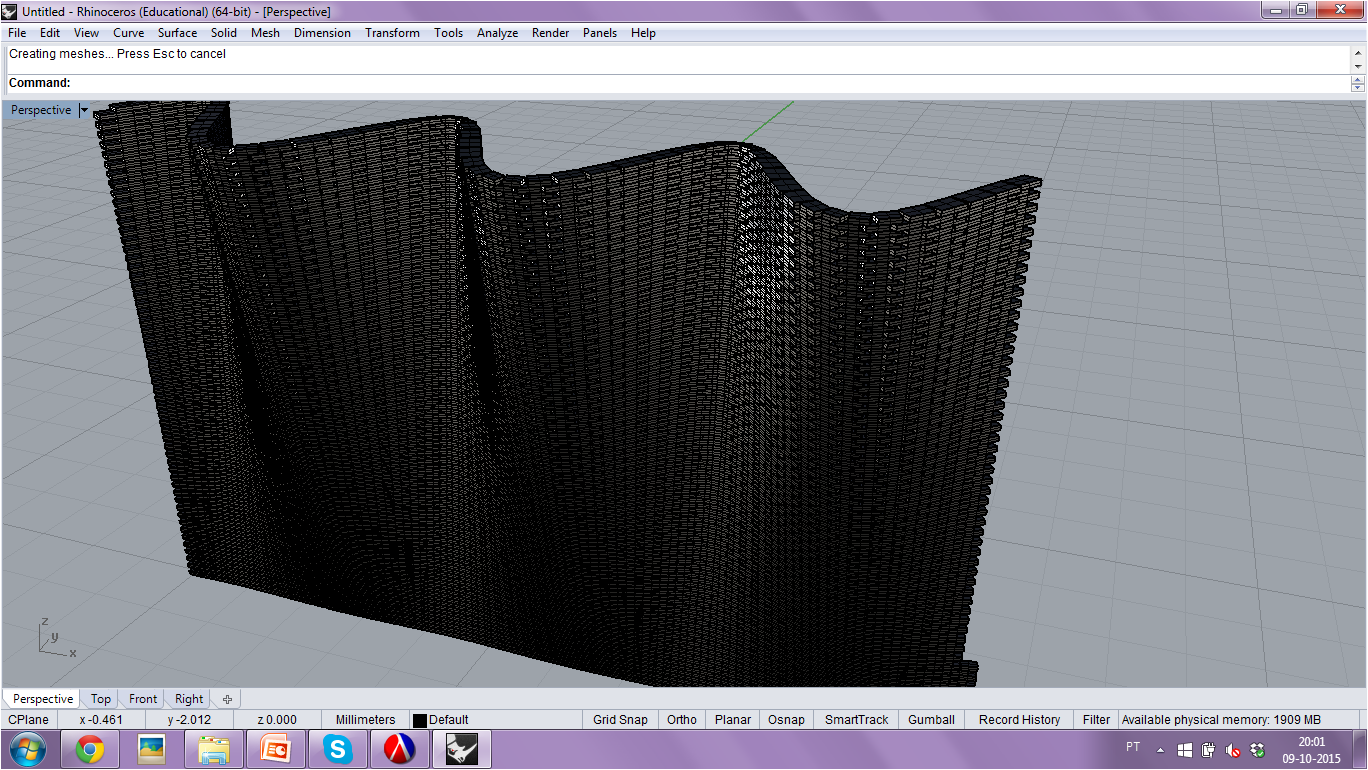
\includegraphics[width=0.7\textwidth, trim = 20mm 25mm 80mm 28mm, clip]{images/parede-sin.png}
	\caption{Wall of bricks}
	\label{fig:brickwall}
\end{figure}


%In this field they also face the problems that raises from the modeling of really big sets of objects and forms manually, which is slow and error prone. 
%\emph{This work addresses the problem of large content creation and will focus on the fields of architecture and design.}

The obvious solution to this problem is to hire more architects or designers in order to increase productivity and reduce the time needed. However, experience has shown that this solution is not scalable, i.e. doubling the number of architects or designers working in a project will not double their overall productivity. Also, this solution has a big impact on financial costs, that would take immediately out of the market producers with fewer resources.

A solution for this problem is the use of \gls{GD}. It is a design method that is based on a programming approach which allows architects and designers to model large volumes of complex shapes with significantly less effort. They can model cities, buildings, trees, and many other objects that are, usually, too big or complex for a manual approach. Since the models are represented by a computer program, large volumes of geometry can be generated within short periods of time. This is positive to the users because it is more efficient than the manual approach, but, in the other hand, it imposes the use of machines with performance that can handle large amounts of geometry fast. The brick wall model (Figure~\ref{fig:brickwall}) can be easily modeled, with a \gls{GD} approach by using a sinusoidal function for the positioning of the bricks. 

Although most \gls{CAD} applications provide programming languages for generative design, programs written in these languages have very limited portability. Additionally, the provided languages, such as AutoLisp, C++ or Visual Basic, are not pedagogical and are difficult to use even to experienced programmers. All this problems create barriers to the adherence to this approach by all users, specially those that are not used to code.\cite{ramos_et_al:OASIcs:2014:4565}

There are several generative design (GD) tools such as Grasshopper\footnote{\url{http://www.grasshopper3d.com/}} and Rosetta\cite{Leit2012}, that aim to break down some of this barriers, and facilitate the approximation of these individuals to programming. With this tools the users can create their models using pedagogical and easy to use languages. This systems implement a straightforward pipeline presented in Figure~\ref{fig:GD_Pipeline}.


%\begin{figure}[htbp]
%	\centering
%	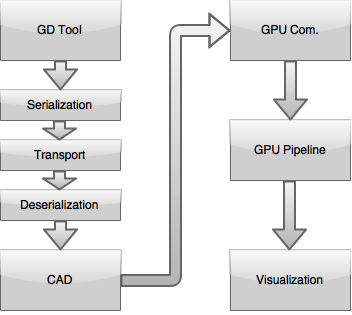
\includegraphics[width=0.45\textwidth]{img/Architecture/GD-Common-Pipeline.png}
%	\caption{Common Generative Design Pipeline}
%	\label{fig:GD_Pipeline}
%\end{figure}

Users implement their models through the GD tool interface. Then all the geometry data is serialized and the data is transfered through some transport mechanism. This data has to be deserialized on the other side within the CAD application. The CAD application takes the deserializes data and processes it producing geometry. Finally, the geometry is moved to the GPU that renders it. All these steps are time-consuming, due to the large amount of data that needs to be transfered. This creates a performance problem.

One big difference between GD and traditional approaches is that users do not see the result of their program while they code. They follow a code-execute-visualize loop where they make changes in the code, execute the code and visualize the resulting model. This makes it difficult for them to understand the impact of changes in their programs. It would be much more productive if they could easily understand the correlation between their program and the resulting model and to be able to experiment values on their program and see the effects they have on the model. To help them with this, there is the concept of \emph{immediate feedback}. Immediate feedback is a mechanism that allows the users to quickly see the results of the changes they make. This can be implemented, for instance, through the use of sliders that can be associated with values on the program, and when one slider is moved the effects of that change should be visualized immediately. 

However, there is a problem: CAD applications are built for manual modeling mainly, and are not prepared to quickly handle large amounts of geometry. Running the code produces much more geometry and much faster than manual modeling, so the user is able to create massive amounts of geometry, which is fed to the CAD that gets overloaded. With this issues, it is hard to get good performance, specially with large models, that makes impossible to have true immediate feedback. There are a lot of techniques that architects and designers may want to use, such as Fractals(Section~\ref{ssub:fractals}), Cellular Automata (Section~\ref{sub:cellular_automaton}), and L-Systems (Section~\ref{ssub:l_systems}), that can generate large amounts of geometry from simple sets of instructions. The use of this techniques are not possible with manual use, due to the large amount of geometry, and is also not possible with the normal pipeline because its performance can not handle the massive amount of geometry that is generated.

% section motivation (end)


%!TEX root = ../../dissertation.tex

\section{Project objectives} % (fold)
\label{sec:project_objectives}


Nowadays new cities are being built  completely from scratch. An example of these cities is the city of Maasdar\footnote{\url{http://www.masdar.ae/en/masdar/detail/masdar-city-free-zone}} in Abu Dhabi. This city, designed by Foster and Partners, is currently being built in the desert at an estimated cost between 18 and 19 billion US\$. Whoever is responsible for a project of this size can not afford to make any mistakes.
To designs this projects it is necessary to create models, but in contrast to the relatively small size of a model of a single building, in this situations an entire city has to be modeled. Therefore, it requires generation and visualization of very large amounts of geometry.

The overall goal of our work is to build a GD tool that solves the performance problems that raise with the generation and visualization of large amounts of geometry. It should be an easy to use tool, with very high performance that will be focused on model visualization, avoiding features regarding interactive model manipulation.

It also should be able to support Immediate Feedback, i.e. allow the users to quickly see the results of the changes they make, for much larger models than the current GD tools can handle. This system should also provide a significant amount of geometric primitives such as \emph{boxes}, \emph{cylinders} or \emph{spheres} that will allow users to model a large variety of shapes.

It will also provide a programming interface, that is how users will interact with the system. It should be simple and easy understand, yet broad and powerful to give the users freedom to create. This will be the visible part of the system together with the visualization window.

After, there is the \textbf{GPU communication} module that implement the functions provided. This module will generate the geometry description, create the windows and transfer the data to the GPU. This module will implement a set of techniques that will 

The \textbf{GPU pipeline} is where the geometry will be generated and is explained in Section~\ref{sub:modern_opengl}.


This work is being developed in the context of the Rosetta that is also a GD tool that helps architects and designers to develop their work procedurally. Rosetta is an extensible IDE based on \textbf{DrRacket} and built in Racket. 

In this context the module will act as a fast preview mode that allows the users to rapidly see the changes they make on their model during their creative process.

On the next section will be explained the architecture of our proposed solution.


This work proposes a solution to this problem and aim to generate large volumes of geometry that is as close as possible to real-time. It does so by jumping over some steps while drastically decreasing the amount of data that is transfered between steps. First we aim to get the geometry as fast as possible to the GPU, so since our goal is just visualization, we jump the CAD layer, eliminating the first communication steps. Another action is to reduce the amount of data that is transferred, by transferring only a very concise description of the geometry, generating the actual geometry on the GPU.
To improve visualization performance, techniques such as Level Of Detail (Section~\ref{ssub:level_of_detail}) and Occlusion Culling (Section~\ref{ssub:occlusion_culling}) are explored.

The processing work for the generation and visualization of the geometry is shared between the \gls{CPU} and the \gls{GPU}. Happens that the work load can be splitted between this two elements in various different ways. And we explore some different ways to aim to have the best performance possible.
The most common solutions assign the large part of the load to the \gls{CPU}, that is responsible for fully generate the geometry which is then sent to the \gls{GPU} that just does pay off.

The simplest and most used load distribution is to assign a large part of it to the \gls{CPU}, where all the geometry is generated which results in a polygon mesh that is fed to the \gls{GPU}. The \gls{GPU} just renders the final result without any processing of the geometry.

It is also possible to give some of the work to the \gls{GPU}. This is done taking advantage of the programmable \gls{GPU}s, where we can use their processing power to manipulate or generate geometry. The \gls{GPU} is able to execute programs, called shaders, that are able to manipulate the geometry that is generated by the \gls{CPU}. With this method, the geometry is generated by the \gls{CPU} but it is changed by the \gls{GPU}. The \gls{GPU} is able to improve detail of the meshes or implement light effects, among other things.

One alternative to the last distribution is to assign a larger part of the processing work to \gls{GPU}. With this distribution the \gls{CPU} creates concise descriptions of the geometry, which is lighter work load, and the \gls{GPU} is responsible for the amplification of the geometry from the descriptions.

The last alternative is to assign most of the work to the \gls{GPU}. With this method, the program that generates the geometry is fully executed by the \gls{GPU}. It is the option that is more complex since all the code have to be written or translated to shader code. Because it runs only on the \gls{GPU}, we can take advantage of the large number of processors that the \gls{GPU}s currently have, and with that get performance improvements.


% section project_objectives (end)
\include{chapters/Overview}
%TEX root = ../dissertation.tex

\chapter{Related Work}
\label{chapter:relatedwork}
Your chapter's content goes here.

%!TEX root = ../dissertation.tex

\chapter{\TheName}
\label{chapter:\TheName}
This Chapter will present our system, \TheName. 

The first section presents the overall architecture of the system we propose as solution. Within the following sections the system components are explained, detailing obstacles, problems and our solution to face them.

%The design phase is very important and this chapter presents it. It will also present the result of the design phase, which is the system architecture.

%!TEX root = ../../dissertation.tex


\section{System Requirements} % (fold)
\label{sec:system_requirements}
This section will present the main design requirements of the system.

It is this system supposed to be used by inexperienced programmers, in particular architects and designers.
...



(IS THIS REALLY NEEDED?)

%ø - Racket API


% section system_requirements (end)


%!TEX root = ../../dissertation.tex


\section{Architecture} % (fold)
\label{sec:architecture}
This section presents the architecture of the system we propose as solution.

The system follows the architecture in Figure~\ref{fig:architecture}.

A module in Racket was Build. This module provides a \gls{API} for the users to describe their models in the Racket Programming Language.
This \gls{API} is implemented in C++ using modern OpenGL. Each of these modules is explained in the following sections.

\subsection{Racket API} % (fold)
\label{sub:racket_api}
Since the focus users for this system are architects and designers, which do not have large programming experience, several design decisions have been made taking this into account. The \gls{PL} that is used by the users is the Racket Programming Language. This is a \gls{PL} that was developed emphasizing pedagogy, is well known for being a good for beginners \cite{Findler1997}\cite{Findler2002}.
The racket module was build to allow the users to implement their models in the Racket Programming Language. 

% subsection racket_api (end)

\subsection{OpenGL Backend} % (fold)
\label{sub:opengl_backend}
We implemented the API with C++ using modern OpenGL. We use this platform with two main reasons, (1) OpenGL is a cross platform API for graphics, and (2) the previous experience with the platform.

% subsection opengl_backend (end)


% section architecture (end)

%!TEX root = ../../dissertation.tex

\section{The System} % (fold)
\label{sec:the_system}

This section explains \TheName further. It presents the problems that we have faced and the respective solutions that we have found to solve them.
As expected, the main problem \TheName aims to solve is about performance. Current tools for \gls{GD} are simply too slow. We attack this problem in a number of fronts. Form diminishing the amount of data that is transferred between layers, to the management of the size of the model that is processed.

\subsection{Transferring Data} % (fold)
\label{sub:transferring_data}

One problem that we encountered on the traditional approaches is the amount of data that is transferred from the GD Tools to the module where it is processed and visualized, usually CAD's. 
%The load that is transfered heavy it was to process all that data that is serialized and deserialized at both ends of the communication channel. 
This is a bottleneck that we aimed to solve.

Our solution to this was to transfer the minimum data possible between modules of the system. To achieve this, instead of sending the whole model description, with every point information (position, color, etc.) we did something different. We send a minimum set of descriptors for each object and generate the model as late as possible within the pipeline. 

For each object we support there is a set of attributes that we need to generate, as described in Figure~\ref{fig:datalayout}. This attributes are an object type, a transformation matrix, the color of the object and a number for the scale. This is a fixed number of data that is sent between layers. This might be a problem for very simple primitives since it some times could fit in less data with the traditional approach. But it is easily compensated with more complex primitives. For instance, the data for the points to model a sphere would be much higher than the data we need for our attributes to describe it.


\begin{table}[]
\centering
\begin{tabular}{|l|l|l|l|}
\hline
\multicolumn{4}{|c|}{19 floats}                                           \\ \hline
matrix (13 floats) & color (3 floats) & type (2 floats) & scale (1 float) \\ \hline
\end{tabular}
\captionof{figure}{Data Layout}\label{fig:datalayout}
\end{table}

% subsection transferring_data (end)

\subsection{Generating Primitives} % (fold)
\label{sub:generating_primitives}

We define primitives as any model that can be modeled by one, description as described in the Section~\ref{sub:transferring_data}.

Since we use a description of the models instead of the whole information, we need to generate the primitives at some point. We do this within the GPU with shaders. More specifically geometry shaders. We support limit set of primitives, all geometric solids, that we believe are able to produce a meaningful set of different models.
Those are: Prisms, Pyramids and Spheres. Note that the prisms include Box's, Cylinders and anything in between.

With this we use simple 3D modeling parametric algorithms to generate the primitives according to the description. This allows us to have the models as late as possible. This fact helps us improve the performance of our system as explained in Section~\ref{sub:size}.

% subsection generating_primitives (end)

\subsection{Model Processing} % (fold)
\label{sub:size}

We aim to support very large models with our system. This means that sometimes, part of the model might be not visible form the current camera position. The \glspl{GPU} are able to cut out this parts of the models when they are processing the faces. This requires that the entire model is generated before it is cut out. For very large models, this process happens too late. For instance, if we have a very large model of a city. It happens that the entire city is behind the camera. The whole model is generated to be after discarded, and this is obviously not good for the performance of the system.

To work on a better solution we take advantage of the timing in which the primitives are generated and apply the Occlusion Culling technique, Section~\ref{sub:occlusion_culling}. When each description of the object is received by the \gls{GPU}, we can know if this object is currently visible form taking into account the position of the camera. With this information we can stop the generation of the object at the beginning, thus generating only the objects that are visible.

Another technique that we implement, and the constant generation of the primitives is that we can manage the Level of Detail at the generation phase.


% subsection performance (end)


\subsection{Transformation} % (fold)
\label{sub:transformation}

Since the objects are generated, we have to implement a transformation solution to generate the object correctly. We tested some options, having as a goal to minimize the number of data needed, this way diminishing the transported data.

\subsubsection{Minimum data} % (fold)
\label{ssub:minimum_data}

First we tried to implement the transformation with the minimum possible data.

Translations and scales can be trivially implemented. By centering the object at a desired point and by creating the objects with an unitary size and then multiplying by the scale, respectively. This two transformations used 3(three) floats each, 6(six) in total. 

For the rotation we implemented the axis-angle representation\cite{curtright2014compact}. This way, we only use 4(four) floats, three for the axis of rotation $\phi$, and the angle $\theta$.

We this solutions we could generate an object with the desired size, rotation and position. 

It happened that the rotation had an issue. The rotation in the axis perpendicular to $\phi$ is undefined, when $\phi$ is not parallel to any of $xyz$ axis. 
Another issue is that this solution is not cumulative. Meaning that we could not create an object and after that, apply any other transformation.

This problems made us look for another solution.

\begin{figure}[h!]
	\centering
	
\includegraphics[width=0.75\textwidth]{images/solution/Axis-Angle_Representation.png}
	\caption{caption}
	\label{fig:axis_angle}
\end{figure}

% subsubsection minimum_data (end)

\subsubsection{Transformation Matrix} % (fold)
\label{ssub:transformation_matrix}

To solve the mentioned problems, we had to compromise on the used data. The previous solution used a total of ten floats to represent the data. 
By using a $4\times4$ matrix we would use six more floats, and could solve both issues.


\begin{figure}[h!]
	\centering
	
\includegraphics[width=0.25\textwidth]{images/solution/Transformation_Matrix.png}
	\caption{caption}
	\label{fig:tmatrix}
\end{figure}

(...)

% subsubsection transformation_matrix (end)



% subsection transformation (end)

\subsection{Adding Color} % (fold)
\label{sub:adding_color}

The assignment of color to the objects was a desired feature, to make \TheName more similar to the other systems. But since we want the minimum amount of data, just adding three more values to transport was not a good solution. To avoid that, we used the last line of the transformation matrix to transport the color values. Thus we could add a totally new feature without adding any more data to transport, just by better using the available space, as shown in Figure~\ref{fig:color_matrix}. This solution makes the data usage gap shorter between the option of having the transformation matrix, Section~\ref{ssub:transformation_matrix}, versus the minimum data option, Section~\ref{ssub:minimum_data}.

\begin{figure}[htbp]
	\centering
	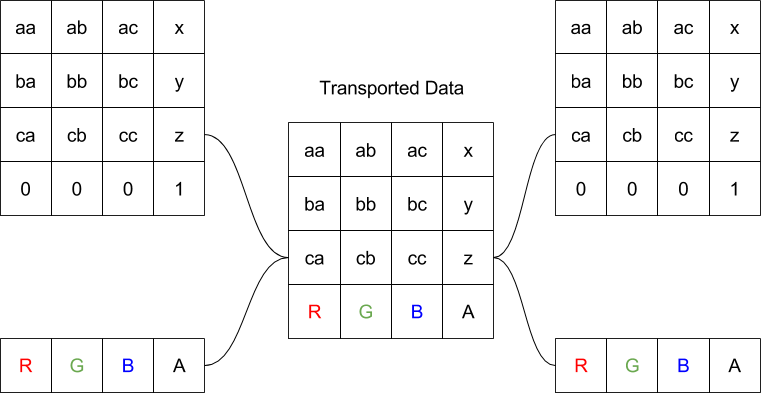
\includegraphics[width=0.95\textwidth]{images/solution/Matrix+Color.png}
	\caption{Transport of the transformation and color data}
	\label{fig:color_matrix}
\end{figure}

% subsection adding_color (end)






% section the_system (end)
%!TEX root = ../dissertation.tex

\chapter{Evaluation}
\label{chapter:evaluation}
Evaluation here...

%!TEX root = ../dissertation.tex

\chapter{Conclusion}
\label{chapter:conclusion}
Conclusion here...



\bibliographystyle{ieeetr}
\addcontentsline{toc}{chapter}{Bibliography}
\bibliography{bibliography/dissertation}

% Appendix
\appendix
%!TEX root = ../dissertation.tex

% Appendix chapters entry point
% Include the chapters below

%!TEX root = ../dissertation.tex

\chapter{Appendix chapter}
\label{appendix:appendix_chapter}



% Glossary and Acronym List
\if\includeGlossary 1
\printglossary
\fi

% Back Cover
\pagenumbering{gobble}
\NewPage

\end{document}
